% Created 2026-04-24 Fri 17:45
% Intended LaTeX compiler: pdflatex
\documentclass[11pt,letterpaper]{report}
\usepackage[utf8]{inputenc}
\usepackage[T1]{fontenc}
\usepackage{graphicx}
\usepackage{longtable}
\usepackage{wrapfig}
\usepackage{rotating}
\usepackage[normalem]{ulem}
\usepackage{amsmath}
\usepackage{amssymb}
\usepackage{capt-of}
\usepackage{hyperref}
\usepackage[margin=1in]{geometry}
\usepackage{titling}
\usepackage{fancyhdr}
\usepackage{tcolorbox}
\usepackage{float}
\pagestyle{fancy}
\fancyfoot[C]{\thepage \quad | \quad SteamPulse — State of Roguelike Deckbuilder — v1.0 — Confidential}
\author{{[}Your name], SteamPulse Research}
\date{{[}Month Year]}
\title{STATE OF ROGUELIKE DECKBUILDER — A SteamPulse Deep Dive\\\medskip
\large \# [TODO: write a one-line subtitle naming the genre's central tension]}
\hypersetup{
 pdfauthor={{[}Your name], SteamPulse Research},
 pdftitle={STATE OF ROGUELIKE DECKBUILDER — A SteamPulse Deep Dive},
 pdfkeywords={},
 pdfsubject={},
 pdfcreator={Emacs 30.2 (Org mode 9.7.11)}, 
 pdflang={English}}
\begin{document}

\maketitle
\part*{At a Glance}
\label{sec:orge5c08ca}
\textbf{At a Glance}

\begin{enumerate}
\item The \#1 friction across the genre — \textbf{Item/Card Pool Dilution Degrades Build Agency at High Unlock Counts} — was mentioned in 12 of the 120 games analyzed.
\item The most-requested feature in player wishlists — \textbf{Randomized Daily/Weekly Runs With Global Leaderboards} — appears in 10 games' reviews.
\item Median player churn occurs at hour \textbf{20}. Primary reason: Build convergence: players identify the dominant strategy or exhaust the effective card/item pool and stop experiencing discovery.
\item The benchmark games that anchor this niche: \textbf{Slay the Spire, Balatro, Monster Train}.
\item The single highest-impact design move per the dev-priorities ranking: \textbf{Ship an item/card pool filter or ban mechanic so players can exclude weak or irrelevant unlocks from appearing in runs} (mentioned by 12 games, effort: medium).
\item Dataset: 120 games analyzed; average positive review \% is 88\%; median review count 853.
\item \# [TODO: write a 7th headline finding, or trim to 6]
\end{enumerate}
\part*{How to read this report}
\label{sec:orgdbfb269}
Roguelike deckbuilder players stop playing when winning stops feeling like discovery — not when they lose.

The genre contract is unusually strict. Slay the Spire set the template: a run fits in a single sitting, card synergies are the primary skill expression, and meta-progression persists between deaths. Balatro extended the contract by proving the scoring ceiling itself can be the endgame. Monster Train demonstrated that a genuinely novel spatial mechanic — three floors of positional defense — earns hundreds of hours on its own. Any game shipping in this niche inherits all three promises on day one: strategic depth, run variety, and a reason to return after every loss.

The games that pull ahead all do the same thing: they reward discovery over execution. Players consistently cite "the first time a build clicked" as their peak moment. The sharpest cross-genre friction is build homogenization after 30–80 hours, when the synergy space feels fully mapped and the item or card pool has been diluted by unlocks. A second axis of friction — present in nearly every report — is RNG that spikes at the exact difficulty tier where players expect their accumulated skill to matter most, converting earned progress into a luck check.

For a developer shipping here: broad viable build diversity and a difficulty curve that rewards reads over rolls are the two investments this audience pays back. Everything else is polish.
\part*{SECTION 1 — THE MARKET}
\label{sec:orgfb72332}

\chapter*{At a Glance — The Market}
\label{sec:org319806b}
\chapter*{Market size and growth}
\label{sec:org352006b}
\begin{figure}[H]
\centering
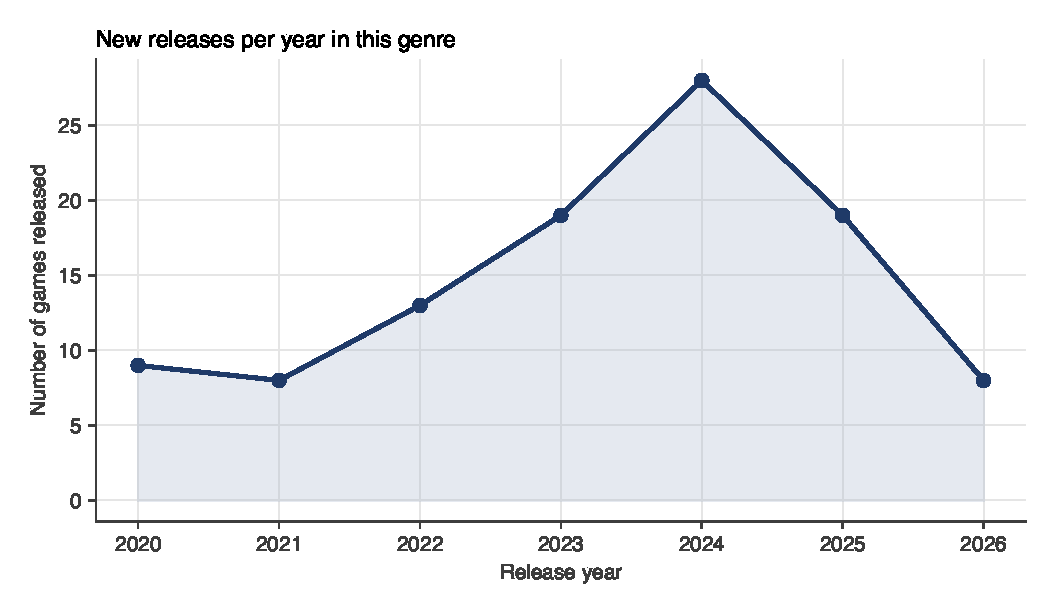
\includegraphics[width=0.9\textwidth]{./charts/releases_per_year.pdf}
\caption{\label{fig:org1df9503}New releases per year in the Roguelike Deckbuilder genre. Source: SteamPulse, release\_date for 120 games, 2026-04-24.}
\end{figure}
\chapter*{Pricing and discounting}
\label{sec:orgb22dc98}
\begin{figure}[H]
\centering
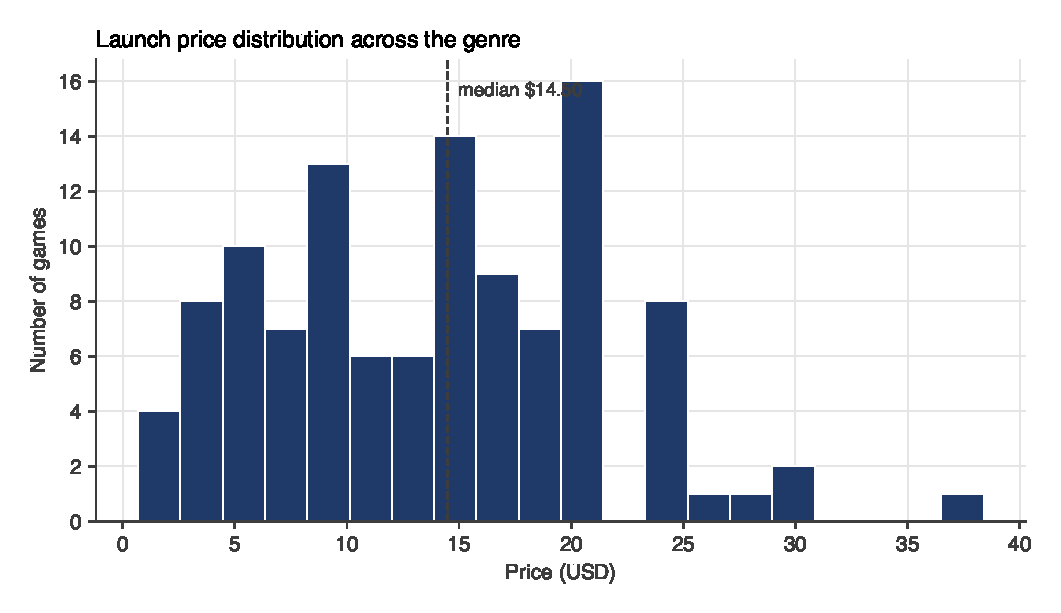
\includegraphics[width=0.9\textwidth]{./charts/price_distribution.pdf}
\caption{\label{fig:orga573aeb}Launch price distribution across Roguelike Deckbuilder games. Source: SteamPulse, current Steam price for 120 games, 2026-04-24.}
\end{figure}
\chapter*{Recent wins and recent losses}
\label{sec:orgcf3e8bb}
\chapter*{Implications for The Market}
\label{sec:org6718cce}
\part*{SECTION 2 — THE PLAYERS}
\label{sec:orgc37df4a}

\chapter*{At a Glance — The Players}
\label{sec:orga246e54}
\chapter*{Who plays this genre}
\label{sec:org486faf3}
\chapter*{The churn wall}
\label{sec:org7421226}
Median player drop-off in this genre occurs at hour \textbf{20}.

The primary reason cited across the dataset:

Build convergence: players identify the dominant strategy or exhaust the effective card/item pool and stop experiencing discovery. Runs feel like execution of a known solution rather than exploration of a possibility space. This is distinct from difficulty frustration — many of these players are winning; they simply have nothing left to find.

\begin{quote}
\emph{After 80–200 hours of completing all content, high-engagement players go dormant waiting for a content update that has no public ETA, converting fans into vocal critics}

— quoted from \emph{Balatro}
\end{quote}
\chapter*{Audience overlap}
\label{sec:org1308496}
\chapter*{Implications for The Players}
\label{sec:org8343dc3}
\part*{SECTION 3 — THE FRICTION \& THE OPPORTUNITY}
\label{sec:orgfadf65a}

\chapter*{At a Glance — Friction \& Opportunity}
\label{sec:org9bbd69a}
\begin{itemize}
\item \textbf{Friction:} Item/Card Pool Dilution Degrades Build Agency at High Unlock Counts (12 games)
\item \textbf{Friction:} RNG Dominates Outcomes at Higher Difficulty Tiers, Undermining Skill Expression (18 games)
\item \textbf{Wishlist:} Randomized Daily/Weekly Runs With Global Leaderboards (10 games)
\item \textbf{Wishlist:} Item Pool Filter or Ban Mechanic to Exclude Weak or Unwanted Unlocks (12 games)
\end{itemize}
\chapter*{Friction clusters}
\label{sec:org4f3bc9d}
\begin{figure}[H]
\centering
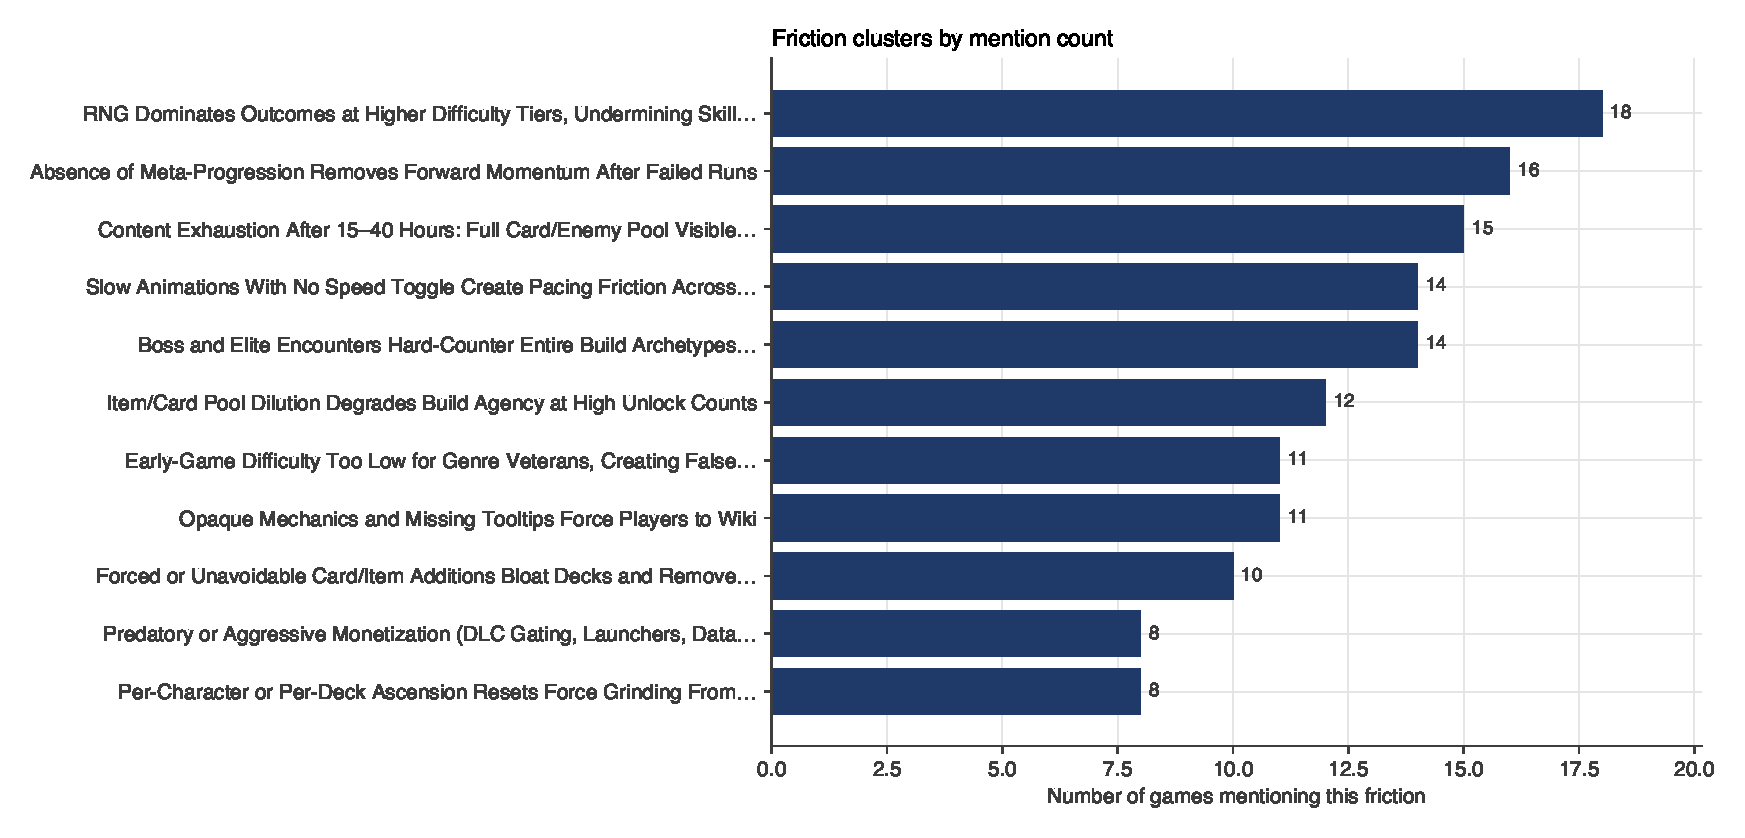
\includegraphics[width=0.9\textwidth]{./charts/friction_counts.pdf}
\caption{\label{fig:org7d2dfc4}Friction clusters in Roguelike Deckbuilder by cross-game mention count. Source: SteamPulse synthesis of 120 games' reviews, 2026-04-24.}
\end{figure}
\section*{Item/Card Pool Dilution Degrades Build Agency at High Unlock Counts}
\label{sec:orgeec62b1}
As players unlock more cards, jokers, or items, the pool expands to include weak options that crowd out viable synergy pieces. Players report that runs become progressively harder to pilot toward an intended build as the pool grows, paradoxically making progression feel like a punishment.

Mentioned in 12 games in the dataset.

\begin{quote}
\emph{Unlocking more jokers dilutes the item pool with weak options, reducing the probability of finding viable builds — and there is no way to filter or disable unlocked items}

— quoted from \emph{Balatro}
\end{quote}
\section*{RNG Dominates Outcomes at Higher Difficulty Tiers, Undermining Skill Expression}
\label{sec:org9aca8f1}
Across virtually every game in the genre, players who invest 20–100 hours and push to higher ascension or difficulty levels report that run outcomes increasingly feel decided by early card/item offerings rather than player decisions, converting what should be a mastery payoff into a luck check.

Mentioned in 18 games in the dataset.

\begin{quote}
\emph{RNG card offerings can produce runs that feel unwinnable from early acts — a consistent complaint from players with 5–64 hours, driving perception of 'luck simulator'}

— quoted from \emph{Slay the Spire}
\end{quote}
\section*{Boss and Elite Encounters Hard-Counter Entire Build Archetypes Without Counterplay}
\label{sec:org733b781}
In multiple titles, specific boss mechanics — ability-disabling, stat-erasing, or build-invalidating phases — arrive without telegraph and negate hours of deck construction. Players describe these as 'instant brick' moments that feel punitive rather than challenging.

Mentioned in 14 games in the dataset.

\begin{quote}
\emph{Doormaker boss is severely overtuned: stacked mechanics (card exhaustion, draw prevention, energy drain, high burst damage) invalidate most deck archetypes and force players to build specifically around it or abandon runs}

— quoted from \emph{Slay the Spire 2}
\end{quote}
\section*{Content Exhaustion After 15–40 Hours: Full Card/Enemy Pool Visible Too Early}
\label{sec:org27a96b2}
Players in mid-tier titles consistently report seeing the complete card pool within two to four runs, at which point the discovery loop — the genre's primary retention driver — collapses. The 'one more run' compulsion requires the possibility of encountering something new.

Mentioned in 15 games in the dataset.

\begin{quote}
\emph{Players hit a build that 'goes infinite' in their first few runs exit within 4–6 hours, concluding the game has no meaningful ceiling}

— quoted from \emph{Luck be a Landlord}
\end{quote}
\section*{Absence of Meta-Progression Removes Forward Momentum After Failed Runs}
\label{sec:org958654c}
Games without any persistent unlock or reward structure between runs see players disengage after content exhaustion or repeated losses, because there is no incremental signal of progress. The genre standard — set by Hades and Slay the Spire — is that every run, win or lose, advances something.

Mentioned in 16 games in the dataset.

\begin{quote}
\emph{The single largest churn driver post-floor-20 is feeling 'done' with nothing to return for. Meta-progression is the structural fix that converts one-time completers into returning players.}

— quoted from \emph{Luck be a Landlord}
\end{quote}
\section*{Slow Animations With No Speed Toggle Create Pacing Friction Across Every Run}
\label{sec:org2e3ae67}
Unskippable or insufficiently fast card play, boss attack, and result animations are a near-universal complaint across the genre. Players who replay content hundreds of times find default pacing multiplies session time without adding value.

Mentioned in 14 games in the dataset.

\begin{quote}
\emph{No animation speed-up option — slow dice-slot and spell-resolve animations make turns and full runs feel significantly longer than equivalent deckbuilder peers, cited by 42 reviewers}

— quoted from \emph{SpellRogue}
\end{quote}
\section*{Forced or Unavoidable Card/Item Additions Bloat Decks and Remove Curation Agency}
\label{sec:org1954f52}
Multiple titles require players to add cards or items after every encounter with no skip, no removal, and no alternative. This directly contradicts the deckbuilder fantasy of intentional construction and is one of the genre's most-cited structural design failures.

Mentioned in 10 games in the dataset.

\begin{quote}
\emph{Deck bloat with no meaningful removal tools — decks balloon to 60+ cards; the only card-removal mechanics add more cards, violating standard deckbuilder conventions}

— quoted from \emph{Cardboard Town}
\end{quote}
\section*{Opaque Mechanics and Missing Tooltips Force Players to Wiki}
\label{sec:orgf3c1246}
Status effects, keyword interactions, and hidden enemy mechanics are consistently underdocumented across the genre. Players describe discovering core rules through deaths rather than UI, creating frustration-dropout in the first 1–3 hours before the strategic layer can hook them.

Mentioned in 11 games in the dataset.

\begin{quote}
\emph{Tutorial and tooltips are insufficient for hidden mechanics: card self-leveling, enchantment vs. tome distinction, and Nomad King unit interactions are discovered only after many hours}

— quoted from \emph{9 Kings}
\end{quote}
\chapter*{Wishlist signals}
\label{sec:orgd6868c2}
\begin{figure}[H]
\centering
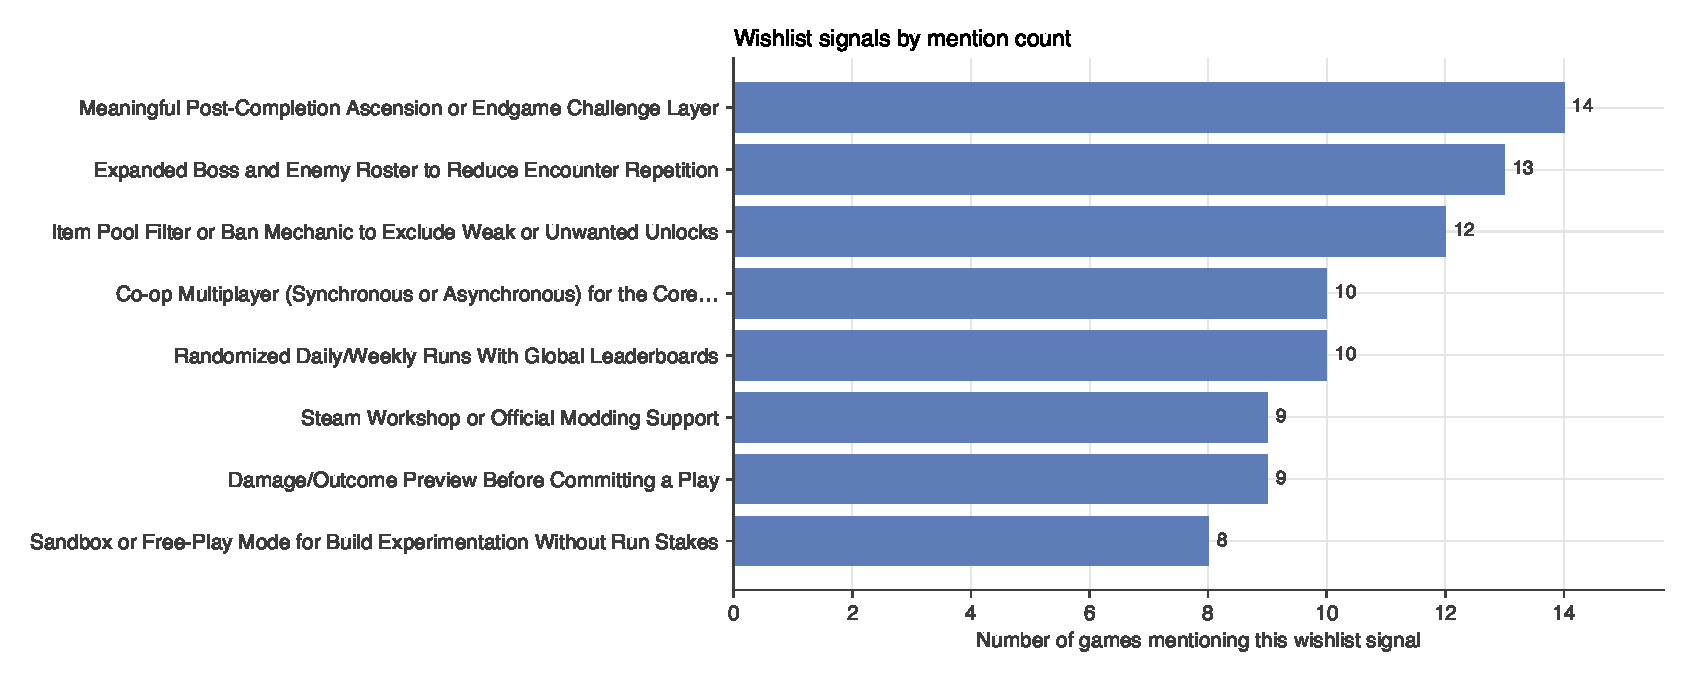
\includegraphics[width=0.9\textwidth]{./charts/wishlist_counts.pdf}
\caption{\label{fig:org1d96920}Wishlist signals in Roguelike Deckbuilder by cross-game mention count. Source: SteamPulse synthesis of 120 games' reviews, 2026-04-24.}
\end{figure}
\section*{Randomized Daily/Weekly Runs With Global Leaderboards}
\label{sec:org824391c}
Players across high-playtime cohorts consistently request seeded daily runs that provide a shared challenge with competitive scoring. This is positioned as the primary reactivation mechanism for players who have exhausted standard content.

Mentioned in 10 games in the dataset.

\begin{quote}
\emph{Randomized daily runs with global leaderboards — the most-requested missing feature among high-playtime players}

— quoted from \emph{Balatro}
\end{quote}
\section*{Item Pool Filter or Ban Mechanic to Exclude Weak or Unwanted Unlocks}
\label{sec:org0de1527}
Players who have unlocked the full game content want control over what appears in their pools, preventing weak or contextually irrelevant items from diluting runs. Vampire Survivors' item locking is frequently cited as the model.

Mentioned in 12 games in the dataset.

\begin{quote}
\emph{Option to filter or exclude specific unlocked jokers from the item pool}

— quoted from \emph{Balatro}
\end{quote}
\section*{Meaningful Post-Completion Ascension or Endgame Challenge Layer}
\label{sec:org4c9e161}
The genre's most engaged players universally want structured post-completion difficulty — a Slay the Spire-style ascension ladder, heat system, or endless modifier stack — that gives a reason to keep running after all content is cleared.

Mentioned in 14 games in the dataset.

\begin{quote}
\emph{Ascension / escalation system (Slay the Spire-style) for structured post-true-ending progression goals}

— quoted from \emph{StarVaders}
\end{quote}
\section*{Co-op Multiplayer (Synchronous or Asynchronous) for the Core Roguelike Loop}
\label{sec:org3c8e8dc}
Players across the genre repeatedly request co-op modes — either full synchronous runs or asynchronous PvP/score challenge. The Slay the Spire 2 co-op implementation is the current reference point generating the strongest positive signal.

Mentioned in 10 games in the dataset.

\begin{quote}
\emph{Co-op multiplayer for up to 4 players adds cross-character synergies and is widely cited as the single biggest upgrade over STS1}

— quoted from \emph{Slay the Spire 2}
\end{quote}
\section*{Damage/Outcome Preview Before Committing a Play}
\label{sec:orge0e140d}
Players in multiple titles request a real-time or pre-commit preview showing how much incoming damage will resolve or what the outcome of a card play will be. Monster Train's damage preview overlay is the most-cited benchmark.

Mentioned in 9 games in the dataset.

\begin{quote}
\emph{Add a damage/consequence preview system showing how much incoming damage will resolve before the player commits a card play}

— quoted from \emph{Wildfrost}
\end{quote}
\section*{Expanded Boss and Enemy Roster to Reduce Encounter Repetition}
\label{sec:org18f3dd9}
Across games with 3–5 bosses and a shallow enemy pool, players with 30+ hours explicitly request additional boss types and elite encounters as the primary content investment that would extend their engagement.

Mentioned in 13 games in the dataset.

\begin{quote}
\emph{More enemy variety — additional elite and boss types per act to reduce rotation fatigue across extended play}

— quoted from \emph{Slay the Spire}
\end{quote}
\chapter*{The promise gap}
\label{sec:orgcb4738f}
\chapter*{Implications for Friction \& Opportunity}
\label{sec:orgc6f1ced}
\part*{SECTION 4 — THE PLAYBOOK}
\label{sec:orged80e9d}

\chapter*{At a Glance — The Playbook}
\label{sec:org4b0352c}
\begin{itemize}
\item Ship an item/card pool filter or ban mechanic so players can exclude weak or irrelevant unlocks from appearing in runs
\item Add an animation speed toggle (minimum 2x, ideally 4x or instant-resolve) as a first-session accessible setting
\item Implement a global or account-level difficulty progression so players exploring new characters or decks do not restart from difficulty 1
\item Design a meaningful meta-progression layer with at minimum a lightweight unlock ladder that rewards every run, win or lose
\end{itemize}
\chapter*{Ranked priorities for builders}
\label{sec:orgdebc19f}
\begin{figure}[H]
\centering
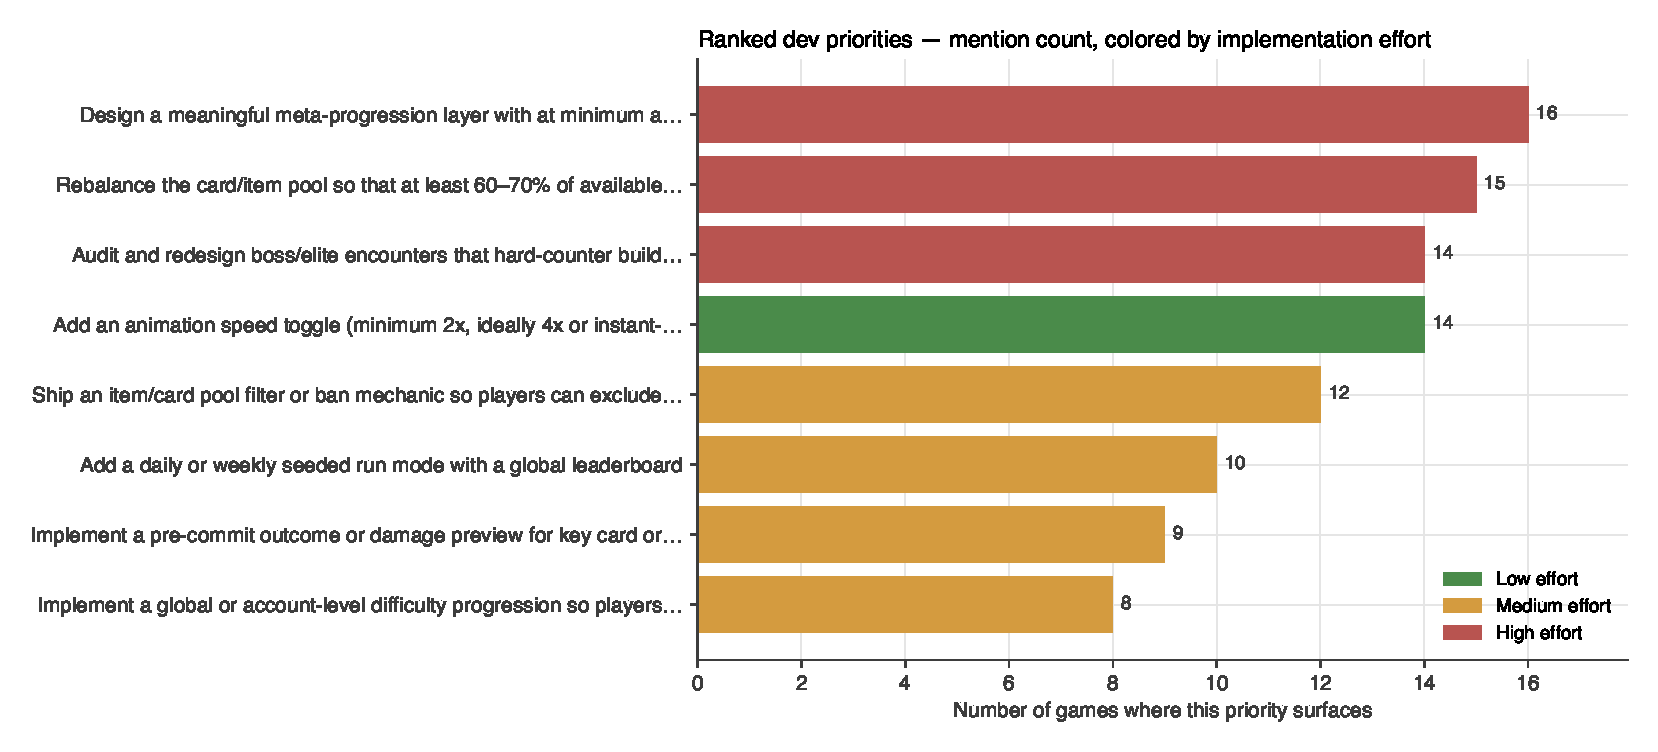
\includegraphics[width=0.9\textwidth]{./charts/dev_priorities.pdf}
\caption{\label{fig:org4ae4025}Ranked dev priorities for Roguelike Deckbuilder — implementation effort vs cross-game demand. Source: SteamPulse synthesis of 120 games' dev\_priorities, 2026-04-24.}
\end{figure}
\section*{1. Ship an item/card pool filter or ban mechanic so players can exclude weak or irrelevant unlocks from appearing in runs}
\label{sec:org18289a6}
\textbf{Effort:} medium | \textbf{Mentioned by:} 12 games

Pool dilution is the single most consistent cross-game friction — it paradoxically makes progression feel like punishment, converting the genre's core retention loop (unlock → more options) into a negative. Every game with a large unlock pool faces this problem, and the fix is table-stakes for long-term replayability.
\section*{2. Add an animation speed toggle (minimum 2x, ideally 4x or instant-resolve) as a first-session accessible setting}
\label{sec:org266718f}
\textbf{Effort:} low | \textbf{Mentioned by:} 14 games

Slow animations are cited in nearly every game in the corpus, always as friction and never as a positive. The cost of this fix is minimal; the retention impact for high-playtime players running their 50th+ session is significant.
\section*{3. Implement a global or account-level difficulty progression so players exploring new characters or decks do not restart from difficulty 1}
\label{sec:orge00960e}
\textbf{Effort:} medium | \textbf{Mentioned by:} 8 games

Per-character ascension resets are the leading structural reason players abandon character variety — the genre's primary replayability axis. The Slay the Spire model (shared ascension unlocked incrementally) is the established solution.
\section*{4. Design a meaningful meta-progression layer with at minimum a lightweight unlock ladder that rewards every run, win or lose}
\label{sec:orgba26437}
\textbf{Effort:} high | \textbf{Mentioned by:} 16 games

The absence of inter-run progression is the primary churn driver in games without it, and the standard has been set by genre leaders. Players who have no incremental signal of progress after a loss have no structural reason to start the next run.
\section*{5. Audit and redesign boss/elite encounters that hard-counter build archetypes without counterplay — replace flat invalidation with readable pressure mechanics}
\label{sec:org4e48270}
\textbf{Effort:} high | \textbf{Mentioned by:} 14 games

Build-invalidating boss encounters appear in the friction data of nearly every game surveyed and are the top driver of run-abandonment at peak investment (30–90 minutes into a run). These are the moments that convert fans into negative reviewers.
\section*{6. Add a daily or weekly seeded run mode with a global leaderboard}
\label{sec:orgea4b4d2}
\textbf{Effort:} medium | \textbf{Mentioned by:} 10 games

This is the single most-requested feature across high-playtime player cohorts in multiple games (Balatro, Slay the Spire, Monster Train 2, SpellRogue). It reactivates dormant players who have cleared base content and provides recurring organic community touchpoints.
\section*{7. Rebalance the card/item pool so that at least 60–70\% of available options are viable in at least one endgame build archetype}
\label{sec:org5b64caa}
\textbf{Effort:} high | \textbf{Mentioned by:} 15 games

Build homogenization — runs converging to 2–5 dominant strategies — is the primary long-term replayability killer across the corpus. Players explicitly name card count and variety as purchase justifications; when the effective pool is a fraction of the total, trust in the game's systems erodes.
\section*{8. Implement a pre-commit outcome or damage preview for key card or ability plays}
\label{sec:orge828978}
\textbf{Effort:} medium | \textbf{Mentioned by:} 9 games

Opaque death states — 'I don't know what killed me' — are a top early-session churn trigger. Monster Train's damage preview is the cited benchmark. This converts frustration-dropout into learning-retention.
\chapter*{Opportunity map}
\label{sec:org4260e37}
\chapter*{What to avoid}
\label{sec:org479083d}
The most common mistakes builders make in this genre — each is the inverse of a friction cluster from Section 3:

\begin{enumerate}
\item \textbf{Don't ship item/card pool dilution degrades build agency at high unlock counts} — see Section 3 for the full pattern. \# [TODO: add a specific game that fell into this trap, with one quote.]
\item \textbf{Don't ship rng dominates outcomes at higher difficulty tiers, undermining skill expression} — see Section 3 for the full pattern. \# [TODO: add a specific game that fell into this trap, with one quote.]
\item \textbf{Don't ship boss and elite encounters hard-counter entire build archetypes without counterplay} — see Section 3 for the full pattern. \# [TODO: add a specific game that fell into this trap, with one quote.]
\item \textbf{Don't ship content exhaustion after 15–40 hours: full card/enemy pool visible too early} — see Section 3 for the full pattern. \# [TODO: add a specific game that fell into this trap, with one quote.]
\item \textbf{Don't ship absence of meta-progression removes forward momentum after failed runs} — see Section 3 for the full pattern. \# [TODO: add a specific game that fell into this trap, with one quote.]
\end{enumerate}
\chapter*{Implications for The Playbook}
\label{sec:orgefd4793}
\part*{APPENDIX A — Benchmark game profiles}
\label{sec:org51b3f50}
\begin{figure}[H]
\centering
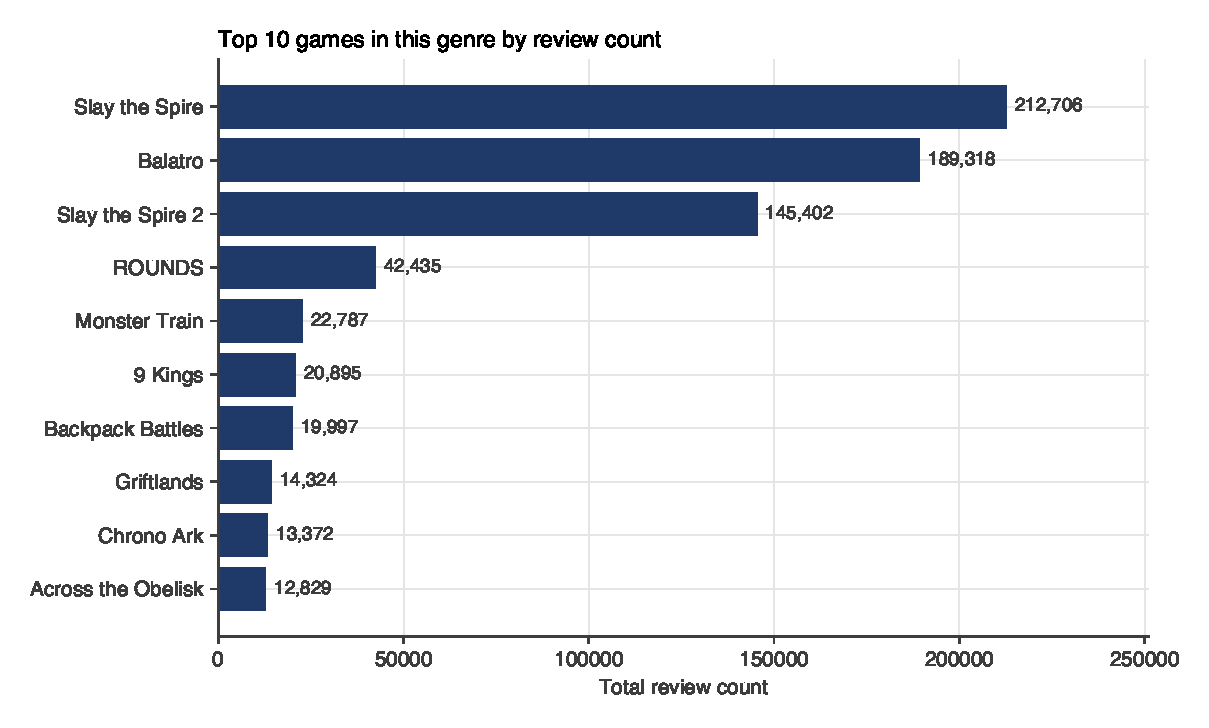
\includegraphics[width=0.9\textwidth]{./charts/top_games_by_reviews.pdf}
\caption{\label{fig:orgfb6edaa}Top 10 games in Roguelike Deckbuilder by total Steam review count. Source: SteamPulse, Steam review\_count data, 2026-04-24.}
\end{figure}
\chapter*{Slay the Spire (appid 646570)}
\label{sec:orgb50c7ba}
The single most-cited reference across the entire input set — present in competitive\_context for nearly every game analyzed. Establishes the genre baseline for card pool depth, ascension difficulty, run pacing, and the standard against which all other deckbuilders are measured.
\chapter*{Balatro (appid 2379780)}
\label{sec:orgd773597}
The second most frequently referenced game across the input corpus, cited as a peer or aspirational comparison in dozens of reports. Represents the current ceiling for accessible deckbuilder design: high player agency, exceptional dopamine loop, and the 'scoring ceiling as endgame' innovation.
\chapter*{Monster Train (appid 1102190)}
\label{sec:org16a56eb}
Appears in competitive\_context for the majority of input reports, consistently cited as the top-tier alternative to Slay the Spire. Establishes the standard for spatial mechanical differentiation, dual-faction combinatorics, and run pacing in the 30–60 minute sweet spot.
\chapter*{Slay the Spire 2 (appid 2868840)}
\label{sec:org3e0c3ac}
Heavily referenced in reports from late 2025 and 2026, cited as the current active benchmark for co-op deckbuilding and as a direct replacement signal for multiple games in the corpus. Its April patch controversy is the most widely discussed live-balance event in the dataset.
\chapter*{Hades (appid 1016730)}
\label{sec:org2c9bfd5}
Consistently invoked across the input corpus — not as a direct deckbuilder but as the benchmark for meta-progression design, narrative-in-roguelike integration, and the 'every run advances something' design principle that players cite when criticizing absent persistence systems.
\part*{APPENDIX B — Methodology}
\label{sec:orgfc9f896}
This report synthesizes player-stated signal from \textbf{120 games} tagged "Roguelike Deckbuilder" on Steam, analyzed via the SteamPulse 3-phase LLM pipeline (prompt\_version=v1). Synthesis computed: 2026-04-24.

\textbf{Coverage:}
\begin{itemize}
\item Games included: 120 (full list in Appendix C)
\item Average positive-review percentage across the dataset: 88\%
\item Median review count per included game: 853
\end{itemize}

\begin{figure}[H]
\centering
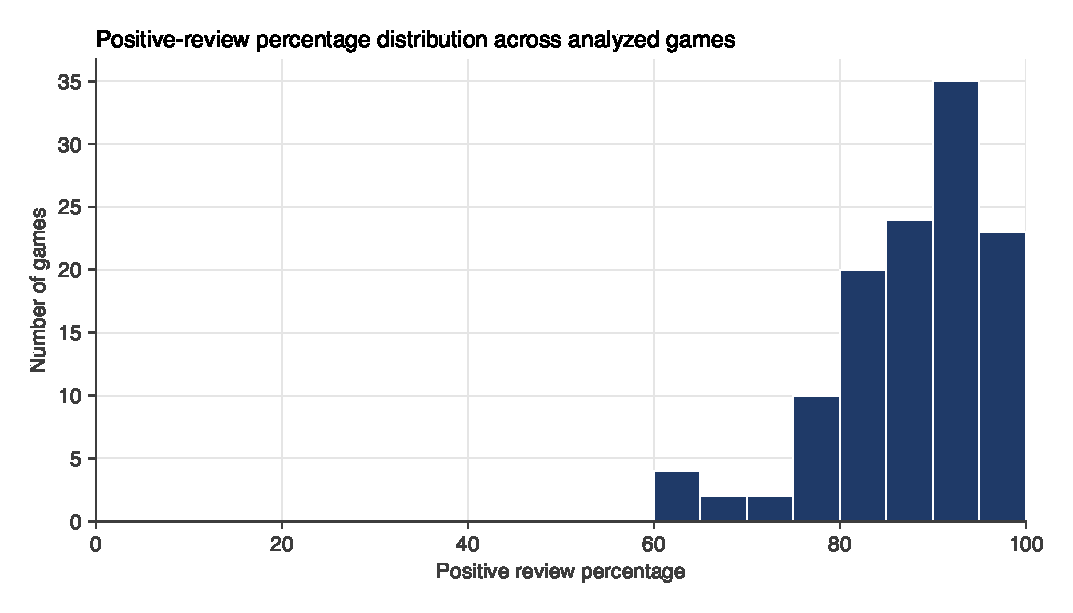
\includegraphics[width=0.9\textwidth]{./charts/positive_pct_distribution.pdf}
\caption{\label{fig:org16f0c60}Distribution of Steam positive-review percentages across the 120 games analyzed. Source: SteamPulse, Steam review\_score data, 2026-04-24.}
\end{figure}
\part*{APPENDIX C — Games included in this analysis}
\label{sec:org408b213}
\begin{center}
\begin{tabular}{rlrl}
Appid & Name & Reviews & Positive \%\\
\hline
646570 & Slay the Spire & 212706 & 98\%\\
2379780 & Balatro & 189318 & 98\%\\
2868840 & Slay the Spire 2 & 145402 & 94\%\\
1557740 & ROUNDS & 42435 & 96\%\\
1102190 & Monster Train & 22787 & 97\%\\
2784470 & 9 Kings & 20895 & 93\%\\
2427700 & Backpack Battles & 19997 & 93\%\\
601840 & Griftlands & 14324 & 93\%\\
1188930 & Chrono Ark & 13372 & 94\%\\
1385380 & Across the Obelisk & 12829 & 82\%\\
861540 & Dicey Dungeons & 11539 & 90\%\\
1404850 & Luck be a Landlord & 11373 & 94\%\\
769560 & 月圆之夜 (Night of Full Moon) & 10873 & 80\%\\
266510 & Hand of Fate & 10641 & 88\%\\
449960 & Book of Demons & 9456 & 89\%\\
2742830 & Monster Train 2 & 9390 & 96\%\\
1811990 & Wildfrost & 8635 & 92\%\\
1970580 & Backpack Hero & 8318 & 88\%\\
2084000 & Shogun Showdown & 6646 & 97\%\\
981430 & Gordian Quest & 5935 & 88\%\\
456670 & Hand of Fate 2 & 5762 & 84\%\\
2289750 & Super Fantasy Kingdom & 5487 & 89\%\\
1108370 & Ratropolis & 5485 & 87\%\\
2501600 & DICEOMANCER & 5469 & 95\%\\
2719030 & Meme Mayhem & 5052 & 92\%\\
998740 & Ring of Pain & 5027 & 92\%\\
3444020 & Demonic Mahjong & 4976 & 96\%\\
1201540 & HELLCARD & 4546 & 87\%\\
1755830 & Astrea: Six-Sided Oracles & 4438 & 93\%\\
1076200 & Roguebook & 4352 & 84\%\\
1919460 & Seraph's Last Stand & 4302 & 89\%\\
2179850 & Cobalt Core & 4164 & 97\%\\
2097570 & StarVaders & 4028 & 98\%\\
2181610 & Heretic's Fork & 4006 & 86\%\\
3052450 & Morimens & 3901 & 88\%\\
1668690 & Alina of the Arena & 3889 & 93\%\\
1793250 & Take Me To The Dungeon!! & 3838 & 91\%\\
1265820 & Fights in Tight Spaces & 3808 & 92\%\\
2824490 & He is Coming & 3760 & 87\%\\
2693930 & Dice \& Fold & 3668 & 83\%\\
2459550 & Emberward & 3640 & 97\%\\
2738490 & Sol Cesto & 3490 & 90\%\\
2356780 & Dungeon Clawler & 3426 & 93\%\\
3784030 & RACCOIN: Coin Pusher Roguelike & 3376 & 87\%\\
2400510 & Dungeons \& Degenerate Gamblers & 3313 & 84\%\\
1038370 & Trials of Fire & 3240 & 88\%\\
1075740 & Banners of Ruin & 3185 & 79\%\\
919370 & Overdungeon & 3103 & 79\%\\
1135810 & Vault of the Void & 2954 & 94\%\\
698640 & Deep Sky Derelicts & 2860 & 73\%\\
1232580 & Knock on the Coffin Lid & 2847 & 82\%\\
3265700 & Vampire Crawlers: The Turbo Wildcard from Vampire Survivors & 2803 & 98\%\\
2697930 & Commander Quest & 2800 & 87\%\\
2026820 & Die in the Dungeon & 2767 & 93\%\\
2735630 & Frostrain & 2697 & 89\%\\
317820 & Guild of Dungeoneering Ultimate Edition & 2614 & 75\%\\
2056210 & LONESTAR & 2351 & 90\%\\
2644610 & Menace from the Deep & 2325 & 89\%\\
2198070 & Cardboard Town & 2144 & 71\%\\
1140150 & Touhou: Lost Branch of Legend & 1992 & 98\%\\
1260590 & Hadean Tactics & 1860 & 90\%\\
2870340 & Decktamer & 1789 & 91\%\\
1337890 & Choice of Life: Middle Ages & 1784 & 79\%\\
1569090 & Vivid Knight & 1703 & 91\%\\
1803400 & Beneath Oresa & 1666 & 78\%\\
1990110 & SpellRogue & 1590 & 89\%\\
3205380 & Omelet You Cook & 1383 & 99\%\\
2118810 & Breachway & 1366 & 80\%\\
3410180 & Overlooting & 1358 & 81\%\\
1127610 & Iris and the Giant & 1305 & 87\%\\
496620 & Monster Slayers & 1254 & 79\%\\
1711950 & GWENT: Rogue Mage (Single-Player Expansion) & 1246 & 60\%\\
1709900 & Tower Tactics: Liberation & 1229 & 89\%\\
2825880 & Death Howl & 1206 & 93\%\\
1769830 & As We Descend & 1132 & 91\%\\
2113040 & RUNGORE & 1124 & 81\%\\
3617620 & My Card Is Better Than Your Card! & 1085 & 96\%\\
3066570 & Aotenjo: Infinite Hands & 1067 & 95\%\\
1016730 & Deck of Ashes & 1062 & 63\%\\
2917350 & Spin Hero & 1034 & 64\%\\
1996430 & Dicefolk & 983 & 93\%\\
2691350 & .Forty-Five & 973 & 95\%\\
1073320 & Meteorfall: Krumit's Tale & 885 & 92\%\\
2852980 & Necroking & 873 & 76\%\\
920680 & Fate Hunters & 871 & 80\%\\
1054550 & Phantom Rose & 869 & 87\%\\
1142080 & Pawnbarian & 863 & 89\%\\
770100 & One Deck Dungeon & 861 & 79\%\\
2113050 & RUNGORE: Beginner Experience & 858 & 89\%\\
1619570 & Death Roads: Tournament & 793 & 82\%\\
1638390 & Indies' Lies & 781 & 77\%\\
2116060 & Epic Auto Towers & 766 & 69\%\\
2464880 & Terracards & 746 & 86\%\\
1046300 & Pirates Outlaws & 741 & 80\%\\
2019680 & Lewd Gym & 737 & 88\%\\
2468100 & Pyrene & 727 & 90\%\\
2229560 & Zet Zillions & 726 & 90\%\\
930780 & Blood Card & 722 & 81\%\\
2305500 & FAIRY TAIL: DUNGEONS & 719 & 95\%\\
2459750 & Yohane the Parhelion - NUMAZU in the MIRAGE - & 691 & 91\%\\
1389360 & Mech Armada & 678 & 83\%\\
2316330 & Shogun Showdown: Prologue & 678 & 97\%\\
3430340 & Dice A Million & 676 & 90\%\\
1071140 & ORX & 671 & 68\%\\
1766390 & FORWARD: Escape the Fold - Ultimate Edition & 670 & 83\%\\
3435260 & Dice With Death & 651 & 93\%\\
1958340 & Cube Chaos & 614 & 96\%\\
264690 & Coin Crypt & 607 & 84\%\\
1893620 & Circadian Dice & 591 & 94\%\\
2311990 & Rack and Slay & 591 & 91\%\\
2789810 & Bingle Bingle & 575 & 84\%\\
1146230 & DungeonTop & 573 & 83\%\\
463980 & Solitairica & 562 & 75\%\\
3839300 & Dogpile & 558 & 97\%\\
2348090 & Crop Rotation & 546 & 94\%\\
1163740 & Card Hog & 538 & 97\%\\
1709050 & Nitro Kid & 533 & 90\%\\
1494560 & Rogue Voltage & 525 & 97\%\\
3166810 & Insider Trading & 508 & 82\%\\
1434540 & Zoeti & 502 & 60\%\\
\end{tabular}
\end{center}
\part*{APPENDIX D — Glossary}
\label{sec:org8cdb97b}
\part*{About SteamPulse}
\label{sec:org83aad43}

\chapter*{What this report is}
\label{sec:org3f8ad38}
\chapter*{Commission custom research}
\label{sec:orgf6d2417}
\chapter*{Other reports in this series}
\label{sec:org4055c46}
\chapter*{Newsletter}
\label{sec:org5498e44}
\end{document}
